\subsection{Introduction}
%
Microsoft leveraged its constantly-growing worldwide network of data centers to create Azure, a cloud platform that facilitates building, deploying, and managing services and applications, anywhere. 

At its core, Azure is a public cloud computing platform—with solutions including Infrastructure as a Service (IaaS), Platform as a Service (PaaS), and Software as a Service (SaaS) that can be used for services such as analytics, virtual computing, storage, networking, and much more. These services can be used to supplement an on premise server or totally replace it.

A CI-CD architecture is implemented in Microsoft Azure as a culmination of two azure services. Those are 

\begin{itemize}
    \item Azure Portal
    \item Azure DevOps
\end{itemize}

The steps or tasks of a CI-CD pipeline are configured in Azure DevOps service and the application is deployed in a resource inside Azure Portal. However, there is also options to deploy the application in other places such as AWS, GCP or even on-premise server. 
%

\subsection{Azure Portal}
%
The Azure portal is a web-based, graphical user-interface console that works as an alternative to cli tools. With the help of Azure portal, it's possible to manage all the resources in an Azure subscription. For instance, a user can build, test and deploy everything from simple web applications to complex cloud deployments. It also provides custom dashboards for an organized view of resources and tool like azure monitor to inspect the performance of an application.

The main strength of Azure portal is continuous availability. It has an instance available in every Azure data-center, which makes the Azure portal immune to individual failures. The Azure portal also updates continuously and requires no downtime for maintenance activities.\footnote{\url{https://docs.microsoft.com/en-us/azure/azure-portal/azure-portal-overview}}
%

\subsection{Azure DevOps}
%
The Azure DevOps platform is a platform created by Microsoft as a software-as-a-service(SaaS) that provides a tool-set with an end to end DevOps environment for developing, integrating and deploying software on a continuous integration and a continuous deployment pipelines. It promotes a culture and set of practices  that bring all stakeholder together to complete software development and release process. 

Moreover it integrates with almost any industry leading DevOps tools available in the marketplace, such as Docker Registry, Kubernetes, Auzre portal, Terraform, Ansible, GitHub etc.\footnote{\url{https://www.devopsgroup.com/insights/resources/tutorials/all/what-is-azure-devops/}}
%

\subsection{Azure DevOps Key Services}
%
The Azure DevOps platform consists of a few key services such as:\footnote{\url{https://www.simplilearn.com/azure-devops-article}}
\begin{itemize}
    \item Azure Boards
    \item Azure Repos
    \item Azure Pipelines
    \item Azure Test Plans
    \item Azure Artifacts
\end{itemize}
%

\subsubsection{Azure Boards}
%
Azure boards is a service of Azure DevOps through which it is possible to manage a project throughout the entire development life-cycle. It provides the functionality to track tasks, work status, user stories, backlogs, features, and track bugs and defects that are noticed in the project. The three basic work items of azure boards are Epics, Issues, and Task.\footnote{\url{https://www.c-sharpcorner.com/article/azure-devops-boards/}}
%
\subsubsection{Azure Repos}
%
Azure DevOps Repos are a set of repositories that provides the functionality of version control and managing a projects code. It helps to work and coordinate code changes across team. It will allow users to to monitor code, solutions, builds, commits, pushes, Pull requests and branching information about projects. 

Azure Repos provides two types of version control:

\begin{itemize}
    \item Git : distributed version control
    \item Team Foundation Version Control : centralized version control
\end{itemize}
% 

\subsubsection{Azure Pipelines}
%
Azure Pipelines is a service that caters the need for creating pipelines on Azure Cloud Platform so that it's possible to build, test and deploy code project automatically. There are three key distinct advantages of using Azure DevOps pipelines:\footnote{\url{https://docs.microsoft.com/en-us/azure/devops/pipelines/get-started/what-is-azure-pipelines?view=azure-devops}}

 \begin{enumerate}
     \item Version Control System : Azure Pipelines integrates with GitHub, GitHub Enterprise, Azure Repos Git, TFVC, Bitbucket Cloud and Subversion.
     \item Language and application types : Azure Pipeline is compatible with most application types and languages, such as Java, JavaScript, Node.js, Python, .Net, C++, Go, PHP, etc.
     \item Deployment Target :  Azure Pipelines can be used to deploy project code to multiple targets. such as, container registries, virtual machines, Azure services, or any on-premises or cloud target.
 \end{enumerate}
 
 Azure Pipeline is based on a few concepts, which are represented by a few keyword. Such as:
 
 \begin{itemize}
     \item Pipeline: A workflow that defines how test, build, and deployment steps are run.
     \item Stage: It can be used to mark the separation of concerns. Each stage contains one or more jobs.
     \item Job: A stage can contain one or more jobs. Each job runs on an agent.
     \item Step: The smallest building block of a pipeline. It can either be a script or a task.
     \item Agent and Agent pools: An agent is an install-able software that runs one job at a time. Agent pool handles multiple agents.
     \item Artifact: It is a collection of files or packages published by a run. The Artifact is made available to subsequent tasks, such as distribution or deployment.
     \item Trigger: Trigger tells the pipeline when to run.
     \item Environment: It is a collection of resources, where the application is deployed.
     \item Runs: It represents a single execution of a pipeline and collects the logs associated with running the steps and the results of running tests.
 \end{itemize}
%

\subsubsection{Azure Test Plans}
%
Azure Test Plan is a browser-based test management solution for exploratory, planned manual, and user acceptance testing. It provides a browser extension for exploratory testing and gathering feedback from stakeholders. Test Plans are an incredible place for a development team to do their manual testing.\footnote{\url{https://docs.microsoft.com/en-us/azure/devops/test/create-a-test-plan?view=azure-devops}}

For automated testing as part of the CI/CD workflow, Azure Pipelines is the best option. However, Manual and exploratory testing are still significant part of evaluating quality of a product. Azure Test Plans in Azure DevOps provides three main types of test management artifacts: 


\begin{enumerate}
    \item Test plans : Group test suites and individual test cases together
    \item Test suites : Group test cases into separate testing scenarios within a single test plan. 
    \item Test cases : Validate individual parts of the code or app deployment. It can be ensured that the code works correctly, has no errors, and meets business and customer requirements.
\end{enumerate}
%

\subsubsection{Azure Artifacts}
%
Azure Artifacts is an extension that facilitates the discovery, installation and publication of NuGet, NPM and Maven packages in Azure DevOps. It’s highly incorporated with other hubs like Build so that package management can become a smooth part of existing workflows.\footnote{\url{https://azure.microsoft.com/en-us/services/devops/artifacts/}}
%

\subsection{DevOps Workflow Diagram}
%
\begin{figure}[h]
    \centering
    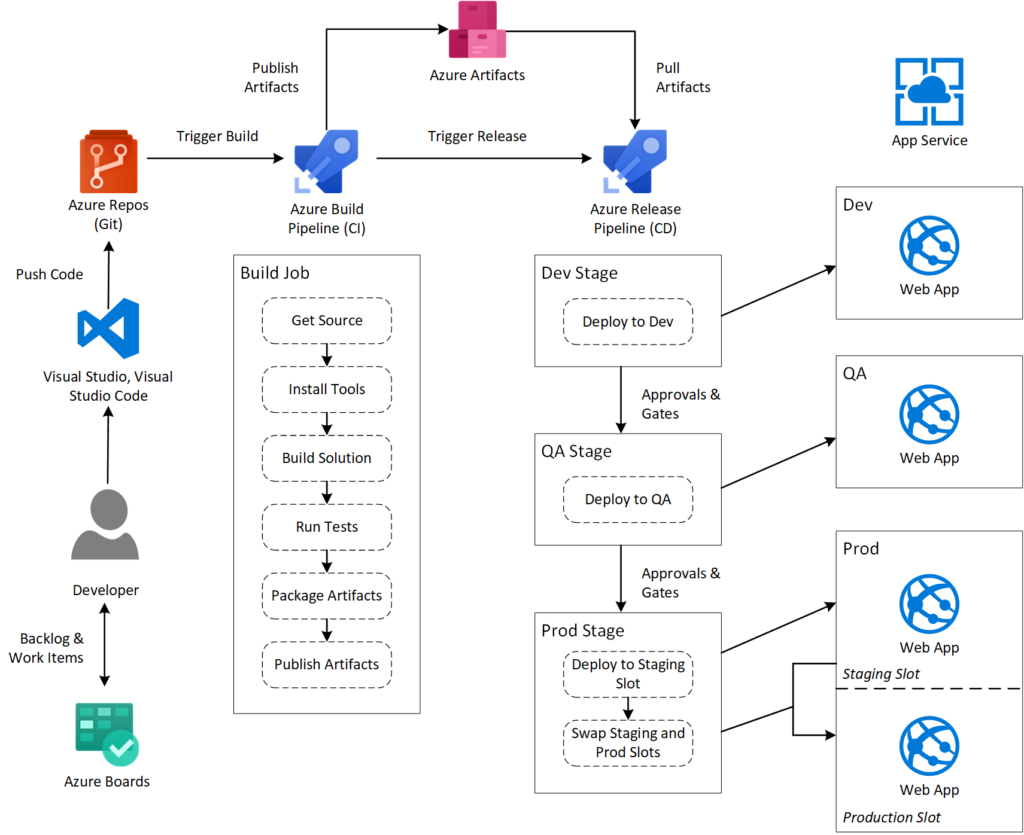
\includegraphics[width=13cm]{images/azure-devops-ci-cd-pipeline-workflow.png}
    \caption{Azure DevOps CI-CD workflow}
    \label{fig:azure-devops-ci-cd-pipeline-workflow}
\end{figure}

In Azure DevOps developers manage and keep track of their tasks and backlogs by using the azure boards service. The source code is developed in a local environment. Azure provides seamless integration with most of the popular IDEs like VS Code, Intellij Idea and Eclipse through extension. Whenever a new commit is pushed to the Azure Repos service it triggers a new build job at Azure Pipelines. A build job can have many stages like installing tools, testing and more. These steps ion a build job can be defined manually by a developer in a azure CI pipeline. After the build is complete, the generated application artifacts are stored in azure artifacts service. Continuous Delivery pipeline is also configured in the azure pipeline service. Whenever a CD pipeline is triggered, it fetches all the necessary artifacts from azure artifacts service and it deploys the application in a pre-configured environment, this environments are used to define and isolate development, QA and production stages in a CI-CD pipeline. These environments are actually stored as a resource groups in azure portal.\footnote{\url{https://www.veritis.com/wp-content/uploads/2019/02/azure-devops-ci-cd-pipeline-flow-veritis-1024x835.png}}

\begin{figure}[h]
    \centering
    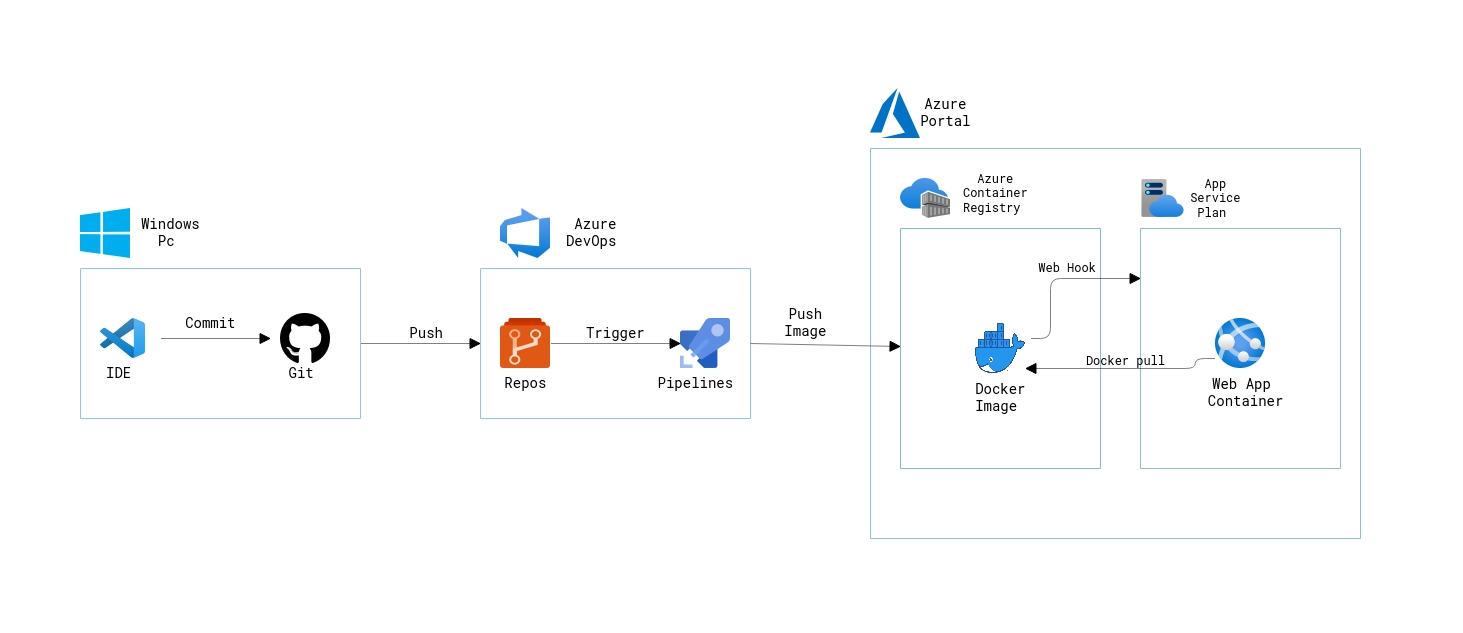
\includegraphics[width=14cm]{images/Azure_pipeline_diagram_CD.png}
    \caption{Azure DevOps CD to Portal}
    \label{fig:azure-devops-ci-cd-pipeline-workflow}
\end{figure}

After CD pipelines are executed the application is continuously deployed in Azure portal. Figure-2 represents a CD-CD pipeline which generates a containerized docker image of the application, this image can be configured to automatically stored in a public registry like DockerHub or Azures own private registry Azure container registry. From where other deployment platform like Azure App service pan, Azure Kubernetes Service (AKS), Azure container instance (ACI) pulls the image through web hooks and deploys the application. All of these steps can be defined by using the azure pipelines service, which will automate the entire system. 
%

\subsection{Advantages}
%
\begin{enumerate}
   \item Since Azure DevOps is a Software-as-a-service(SaaS) product it has many advantages like :\footnote{\url{https://www.softacom.com/en_azure_devops}}
   \begin{itemize}
     \item No manual infrastructure maintenance is needed. 
     \item It is much more intuitively clear and user-friendly in comparison to similar platforms.
     \item Users don’t need to worry about upgrading or patching up the tool-chain, thus massive organizations using the DevOps service will not experience any slowdown in CI-CD pipelines.
   \end{itemize}
   \item Categorized Built in Tasks — In Azure DevOps tasks are categorized based on the nature of operation. For Instance, Build tasks,Utility tasks,Deploy tasks etc. This facilitates user in adding desired tasks to their pipeline in an organized manner.\footnote{\url{https://ymedialabs.medium.com/the-pros-and-cons-of-jenkins-vs-azure-devops-469c66140b4d}}
   \item Group Tasks — It provides the option to encapsulate a sequence of tasks, already defined in a pipeline, into a single reusable task ,just like any other task.
   \item  It is platform agnostic. Which means, Azure DevOps is designed to run on any platform (Linux, macOS, and Windows) or language (e.g., Android, C/C++, Node.js, Python, Java, PHP, Ruby, .Net, and iOS apps).
   \item It is cloud agnostic. That means, Azure DevOps can  work in conjunction with AWS and GCP or even with an on-premise server. 
\end{enumerate}
%

\subsection{Disadvantages}
%
\begin{enumerate}
    \item Azure Pipeline workflow is straightforward. It can’t if-else or switch-case constructions. This makes it more difficult to develop complex workflows.
    \item If the project requires exploratory testing such as alpha,beta testing then the cost structure becomes expensive. 
    \item Documentations of azure are not always up-to-date and sometimes missing.
    \item Integration with non Microsoft tools sometimes can be problematic. 
\end{enumerate}
%

\subsection{Price Plans}
%
   Azure DevOps offers two different plans for purchase :
   \begin{itemize}
     \item Basic Plan : It is free for up-to 5 users, from 6 users on-wards the organization will be charged 6 USD per user every month.
     \item Basic + Test Plans : It costs 52 USD per user per month. 
   \end{itemize}
%